% Template for a Computer Science Tripos Part II project dissertation
\documentclass[12pt,a4paper,oneside,openright]{report}
\usepackage[pdfborder={0 0 0}]{hyperref}    % turns references into hyperlinks
\usepackage[margin=15mm]{geometry}  % adjusts page layout
\usepackage{color}
\usepackage{graphicx}  % allows inclusion of PDF, PNG and JPG images
\usepackage{verbatim}
\usepackage{docmute}   % only needed to allow inclusion of proposal.tex

\usepackage{pdfpages}


\setlength{\parindent}{0ex}

\raggedbottom                           % try to avoid widows and orphans
\sloppy
\clubpenalty1000%
\widowpenalty1000%

\renewcommand{\baselinestretch}{1.1}    % adjust line spacing to make
                                        % more readable



\begin{document}

\bibliographystyle{plain}


%%%%%%%%%%%%%%%%%%%%%%%%%%%%%%%%%%%%%%%%%%%%%%%%%%%%%%%%%%%%%%%%%%%%%%%%
% Title

{\let\cleardoublepage}

\pagestyle{empty}

\rightline{\LARGE \textbf{Marius Latinis}}

\vspace*{60mm}
\begin{center}
\Huge
\textbf{Bus Arrival Time Prediction} \\[5mm]
Computer Science Tripos -- Part II \\[5mm]
Christ's College \\[5mm]
\today  % today's date
\end{center}
\newpage

%%%%%%%%%%%%%%%%%%%%%%%%%%%%%%%%%%%%%%%%%%%%%%%%%%%%%%%%%%%%%%%%%%%%%%%%%%%%%%
% Proforma, table of contents and list of figures

\pagestyle{plain}

\chapter*{Proforma}

{\large
\begin{tabular}{ll}
\textcolor{blue}{Name}: & \bf Marius Latinis                        \\
\textcolor{blue}{College}:            & \bf Christ's College                     \\
\textcolor{blue}{Project Title}:      & \bf Bus Arrival Time Prediction \\
\textcolor{blue}{Examination}:        & \bf Computer Science Tripos -- Part II, July 2017  \\
\textcolor{blue}{Word Count}:         & \bf \textcolor{red}{TODO(ml693): figure out} \\
\textcolor{blue}{Project Originator}: & \bf Dr Richard Mortier \\
\textcolor{blue}{Supervisor}:         & \bf Dr Richard Mortier \\ 
\end{tabular}
}
\stepcounter{footnote}


\section*{Original Aims of the Project}

Implement an algorithm which given the most recent GPS data predicts
when the bus will arrive at the future stops. Evaluate the algorithm
and show that on average it predicts with error less than 80s.

\section*{Work Completed}

All that has been completed appears in this dissertation.

\section*{Special Difficulties}

None
 
\section*{Declaration}

I, Marius Latinis of Christ's College, being a candidate for Part II of the Computer
Science Tripos, hereby declare that this dissertation and the work described 
in it are my own work, unaided except as may be specified below,
and that the dissertation does not contain material that has already been used to any substantial extent for a comparable purpose.

\bigskip
\leftline{Signed [signature]}

\medskip
\leftline{Date \today}

\tableofcontents

%%%%%%%%%%%%%%%%%%%%%%%%%%%%%%%%%%%%%%%%%%%%%%%%%%%%%%%%%%%%%%%%%%%%%%%
% now for the chapters

\pagestyle{headings}

\chapter{Introduction}

\section{Motivation}

In European countries public buses is a popular form of transportation. However,
buses often arrive later than the timetable announces. Therefore, the project aims
to build an algorithm which accuratelly predicts the bus arrival times based on the
most recent GPS data.

\section{Actual Problem Overview}

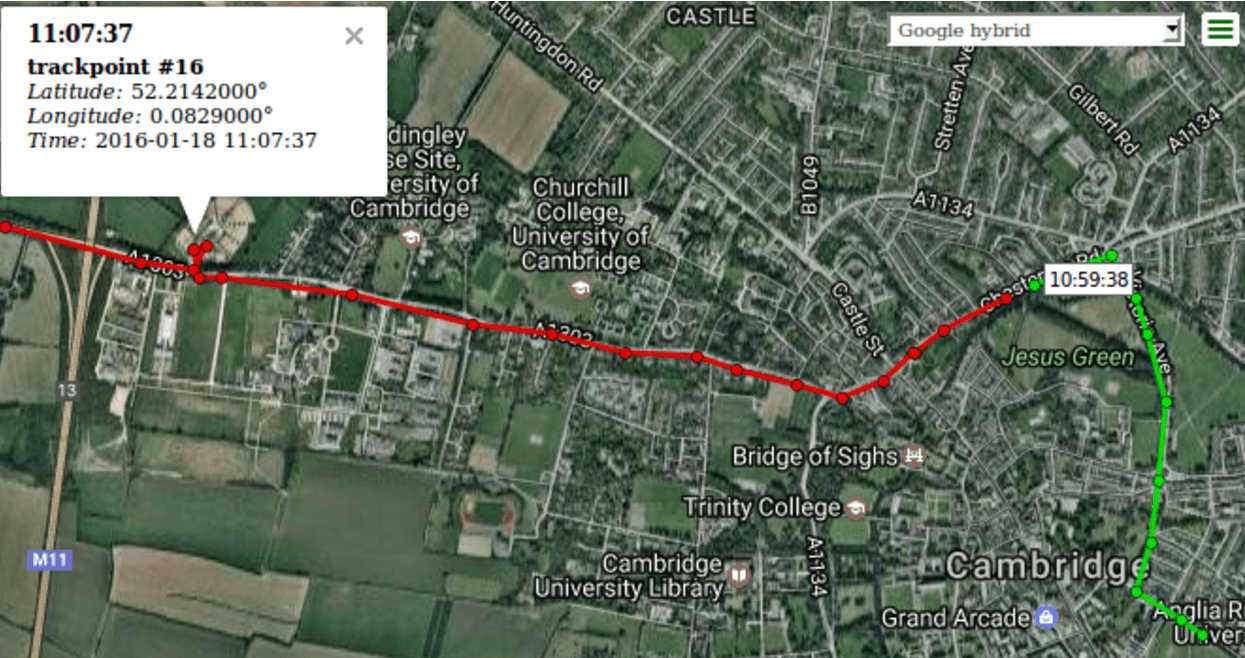
\includegraphics[width=\textwidth]{figs/problem_overview.png} \\


The most recent GPS data (represented by green in the diagram above) shows where the bus has travelled up to now. The future data (represented by red) is not known during the prediction phase. My goal is to predict the future data given the present data. \\

In this specific example I want to predict when the bus will reach Madingley Park 
starting from Chesterton Road. One can see it takes about 8 min. (10:59--11:07)
to travel such distance.

\chapter{Preparation}

\section{Starting Point}
\textcolor{red}{TODO(ml693): put something here}

\section{Preliminary Work}
\textcolor{red}{TODO(ml693): put something here}

{\let\cleardoublepage}
\newpage

\chapter{Implementation}
\
\textcolor{red}{TODO(ml693): replace not my work by my work. The reason
why I am not deleting implementation template yet is because 
it contains nice latex code.}


\section{Verbatim text}

Verbatim text can be included using \verb|\begin{verbatim}| and
\verb|\end{verbatim}|. I normally use a slightly smaller font and
often squeeze the lines a little closer together, as in:

{\renewcommand{\baselinestretch}{0.8}\small
\begin{verbatim}
GET "libhdr"
 
GLOBAL { count:200; all  }
 
LET try(ld, row, rd) BE TEST row=all
                        THEN count := count + 1
                        ELSE { LET poss = all & ~(ld | row | rd)
                               UNTIL poss=0 DO
                               { LET p = poss & -poss
                                 poss := poss - p
                                 try(ld+p << 1, row+p, rd+p >> 1)
                               }
                             }
LET start() = VALOF
{ all := 1
  FOR i = 1 TO 12 DO
  { count := 0
    try(0, 0, 0)
    writef("Number of solutions to %i2-queens is %i5*n", i, count)
    all := 2*all + 1
  }
  RESULTIS 0
}
\end{verbatim}
}

\section{Tables}

\begin{samepage}
Here is a simple example\footnote{A footnote} of a table.

\begin{center}
\begin{tabular}{l|c|r}
Left      & Centred & Right \\
Justified &         & Justified \\[3mm]
%\hline\\%[-2mm]
First     & A       & XXX \\
Second    & AA      & XX  \\
Last      & AAA     & X   \\
\end{tabular}
\end{center}

\noindent
There is another example table in the proforma.
\end{samepage}

\section{Simple diagrams}

Simple diagrams can be written directly in \LaTeX.  For example, see
figure~\ref{latexpic1} on page~\pageref{latexpic1} and see
figure~\ref{latexpic2} on page~\pageref{latexpic2}.

\begin{figure}
\setlength{\unitlength}{1mm}
\begin{center}
\begin{picture}(125,100)
\put(0,80){\framebox(50,10){AAA}}
\put(0,60){\framebox(50,10){BBB}}
\put(0,40){\framebox(50,10){CCC}}
\put(0,20){\framebox(50,10){DDD}}
\put(0,00){\framebox(50,10){EEE}}

\put(75,80){\framebox(50,10){XXX}}
\put(75,60){\framebox(50,10){YYY}}
\put(75,40){\framebox(50,10){ZZZ}}

\put(25,80){\vector(0,-1){10}}
\put(25,60){\vector(0,-1){10}}
\put(25,50){\vector(0,1){10}}
\put(25,40){\vector(0,-1){10}}
\put(25,20){\vector(0,-1){10}}

\put(100,80){\vector(0,-1){10}}
\put(100,70){\vector(0,1){10}}
\put(100,60){\vector(0,-1){10}}
\put(100,50){\vector(0,1){10}}

\put(50,65){\vector(1,0){25}}
\put(75,65){\vector(-1,0){25}}
\end{picture}
\end{center}
\caption{A picture composed of boxes and vectors.}
\label{latexpic1}
\end{figure}

\begin{figure}
\setlength{\unitlength}{1mm}
\begin{center}

\begin{picture}(100,70)
\put(47,65){\circle{10}}
\put(45,64){abc}

\put(37,45){\circle{10}}
\put(37,51){\line(1,1){7}}
\put(35,44){def}

\put(57,25){\circle{10}}
\put(57,31){\line(-1,3){9}}
\put(57,31){\line(-3,2){15}}
\put(55,24){ghi}

\put(32,0){\framebox(10,10){A}}
\put(52,0){\framebox(10,10){B}}
\put(37,12){\line(0,1){26}}
\put(37,12){\line(2,1){15}}
\put(57,12){\line(0,2){6}}
\end{picture}

\end{center}
\caption{A diagram composed of circles, lines and boxes.}
\label{latexpic2}
\end{figure}



\section{Adding more complicated graphics}

The use of \LaTeX\ format can be tedious and it is often better to use
encapsulated postscript (EPS) or PDF to represent complicated graphics.
Figure~\ref{epsfig} and~\ref{xfig} on page \pageref{xfig} are
examples. The second figure was drawn using \texttt{xfig} and exported in
{\tt.eps} format. This is my recommended way of drawing all diagrams.


\begin{figure}[tbh]
\centerline{
\includegraphics{figs/cuarms.pdf}}
\caption{Example figure using encapsulated postscript}
\label{epsfig}
\end{figure}

\begin{figure}[tbh]
\vspace{4in}
\caption{Example figure where a picture can be pasted in}
\label{pastedfig}
\end{figure}


\begin{figure}[tbh]
\centerline{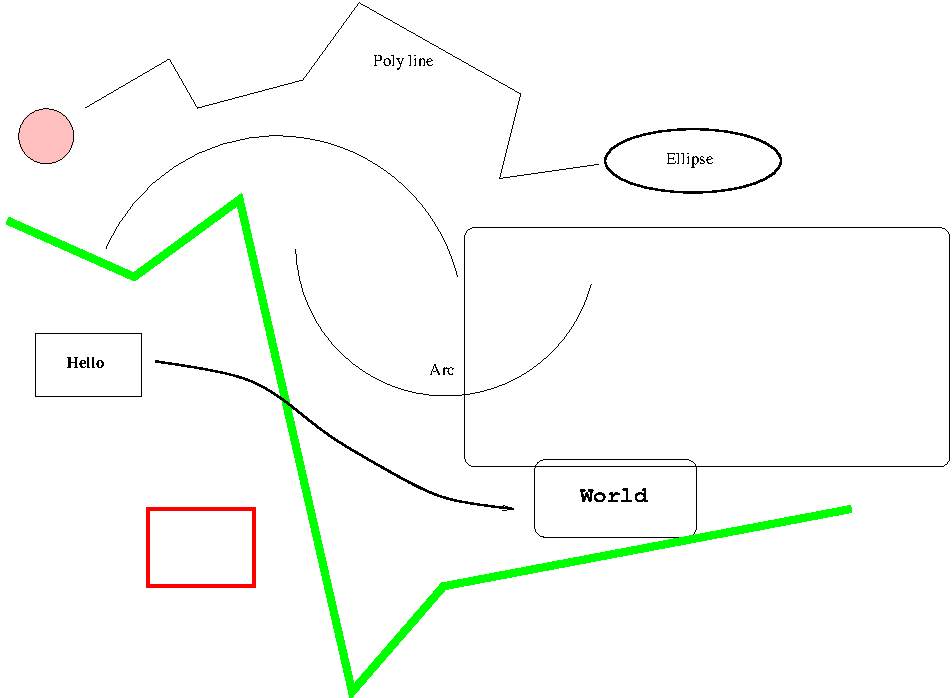
\includegraphics{figs/diagram.pdf}}
\caption{Example diagram drawn using \texttt{xfig}}
\label{xfig}
\end{figure}


\chapter{Evaluation}

\section{Printing and binding}

Use a ``duplex'' laser printer that can print on both sides to print
two copies of your dissertation. Then bind them, for example using the
comb binder in the Computer Laboratory Library.

\section{Further information}

See the Unix Tools notes at

\url{http://www.cl.cam.ac.uk/teaching/current-1/UnixTools/materials.html}


\chapter{Conclusion}

I implemented an algorithm which gives sensible prediction results. The
algorithm itself is simple, thus anyone coming after me to improve the
system should not have trouble read and understand what has been done so far. \\

If started again, I would have worked in exactly the same way.


%%%%%%%%%%%%%%%%%%%%%%%%%%%%%%%%%%%%%%%%%%%%%%%%%%%%%%%%%%%%%%%%%%%%%
% the bibliography
\addcontentsline{toc}{chapter}{Bibliography}
\bibliography{refs}

%%%%%%%%%%%%%%%%%%%%%%%%%%%%%%%%%%%%%%%%%%%%%%%%%%%%%%%%%%%%%%%%%%%%%
% the appendices
\appendix

\chapter{Latex source}

\section{diss.tex}
{\scriptsize\verbatiminput{diss.tex}}

\section{proposal.tex}
{\scriptsize\verbatiminput{proposal.tex}}

\chapter{Makefile}

\section{makefile}\label{makefile}
{\scriptsize\verbatiminput{makefile.txt}}

\section{refs.bib}
{\scriptsize\verbatiminput{refs.bib}}

\chapter{Project Proposal}
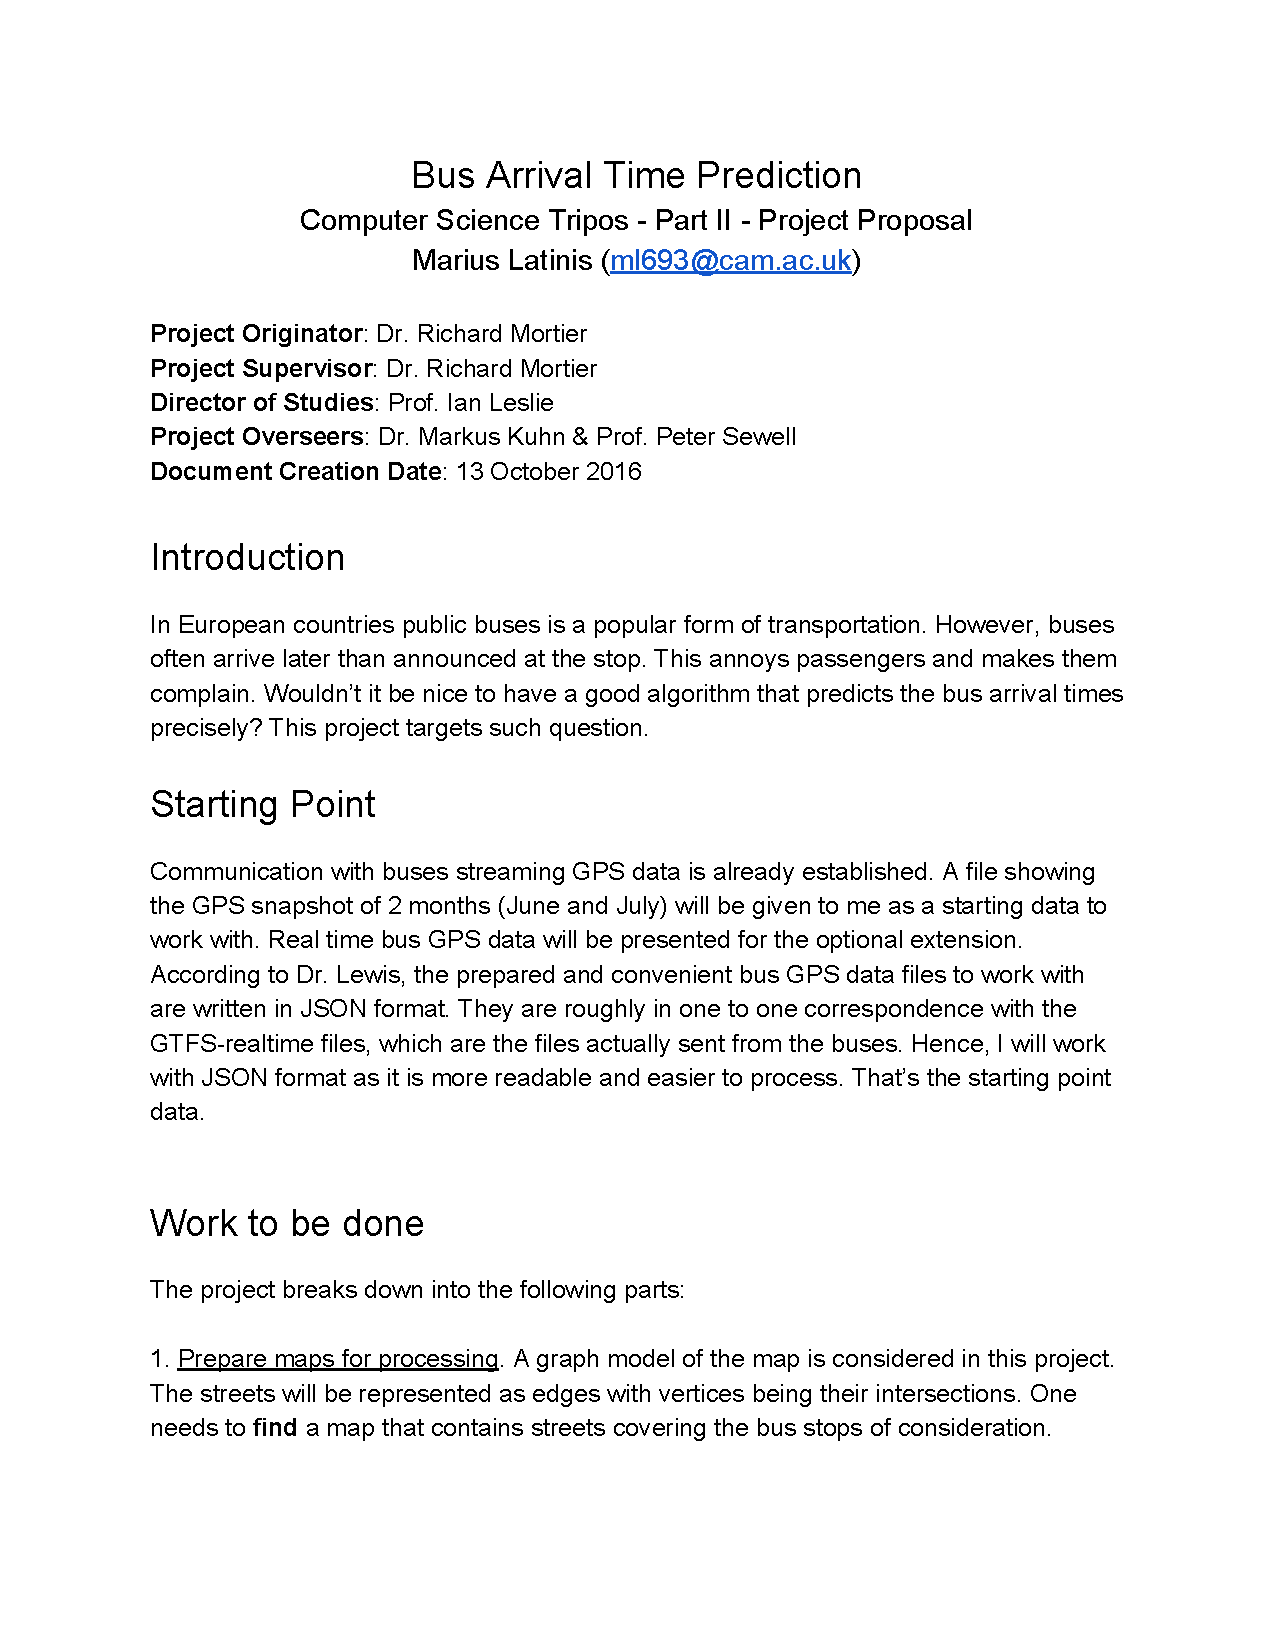
\includepdf[pages=-]{proposal.pdf}

\end{document}
